\begin{figure}[H]
\centering
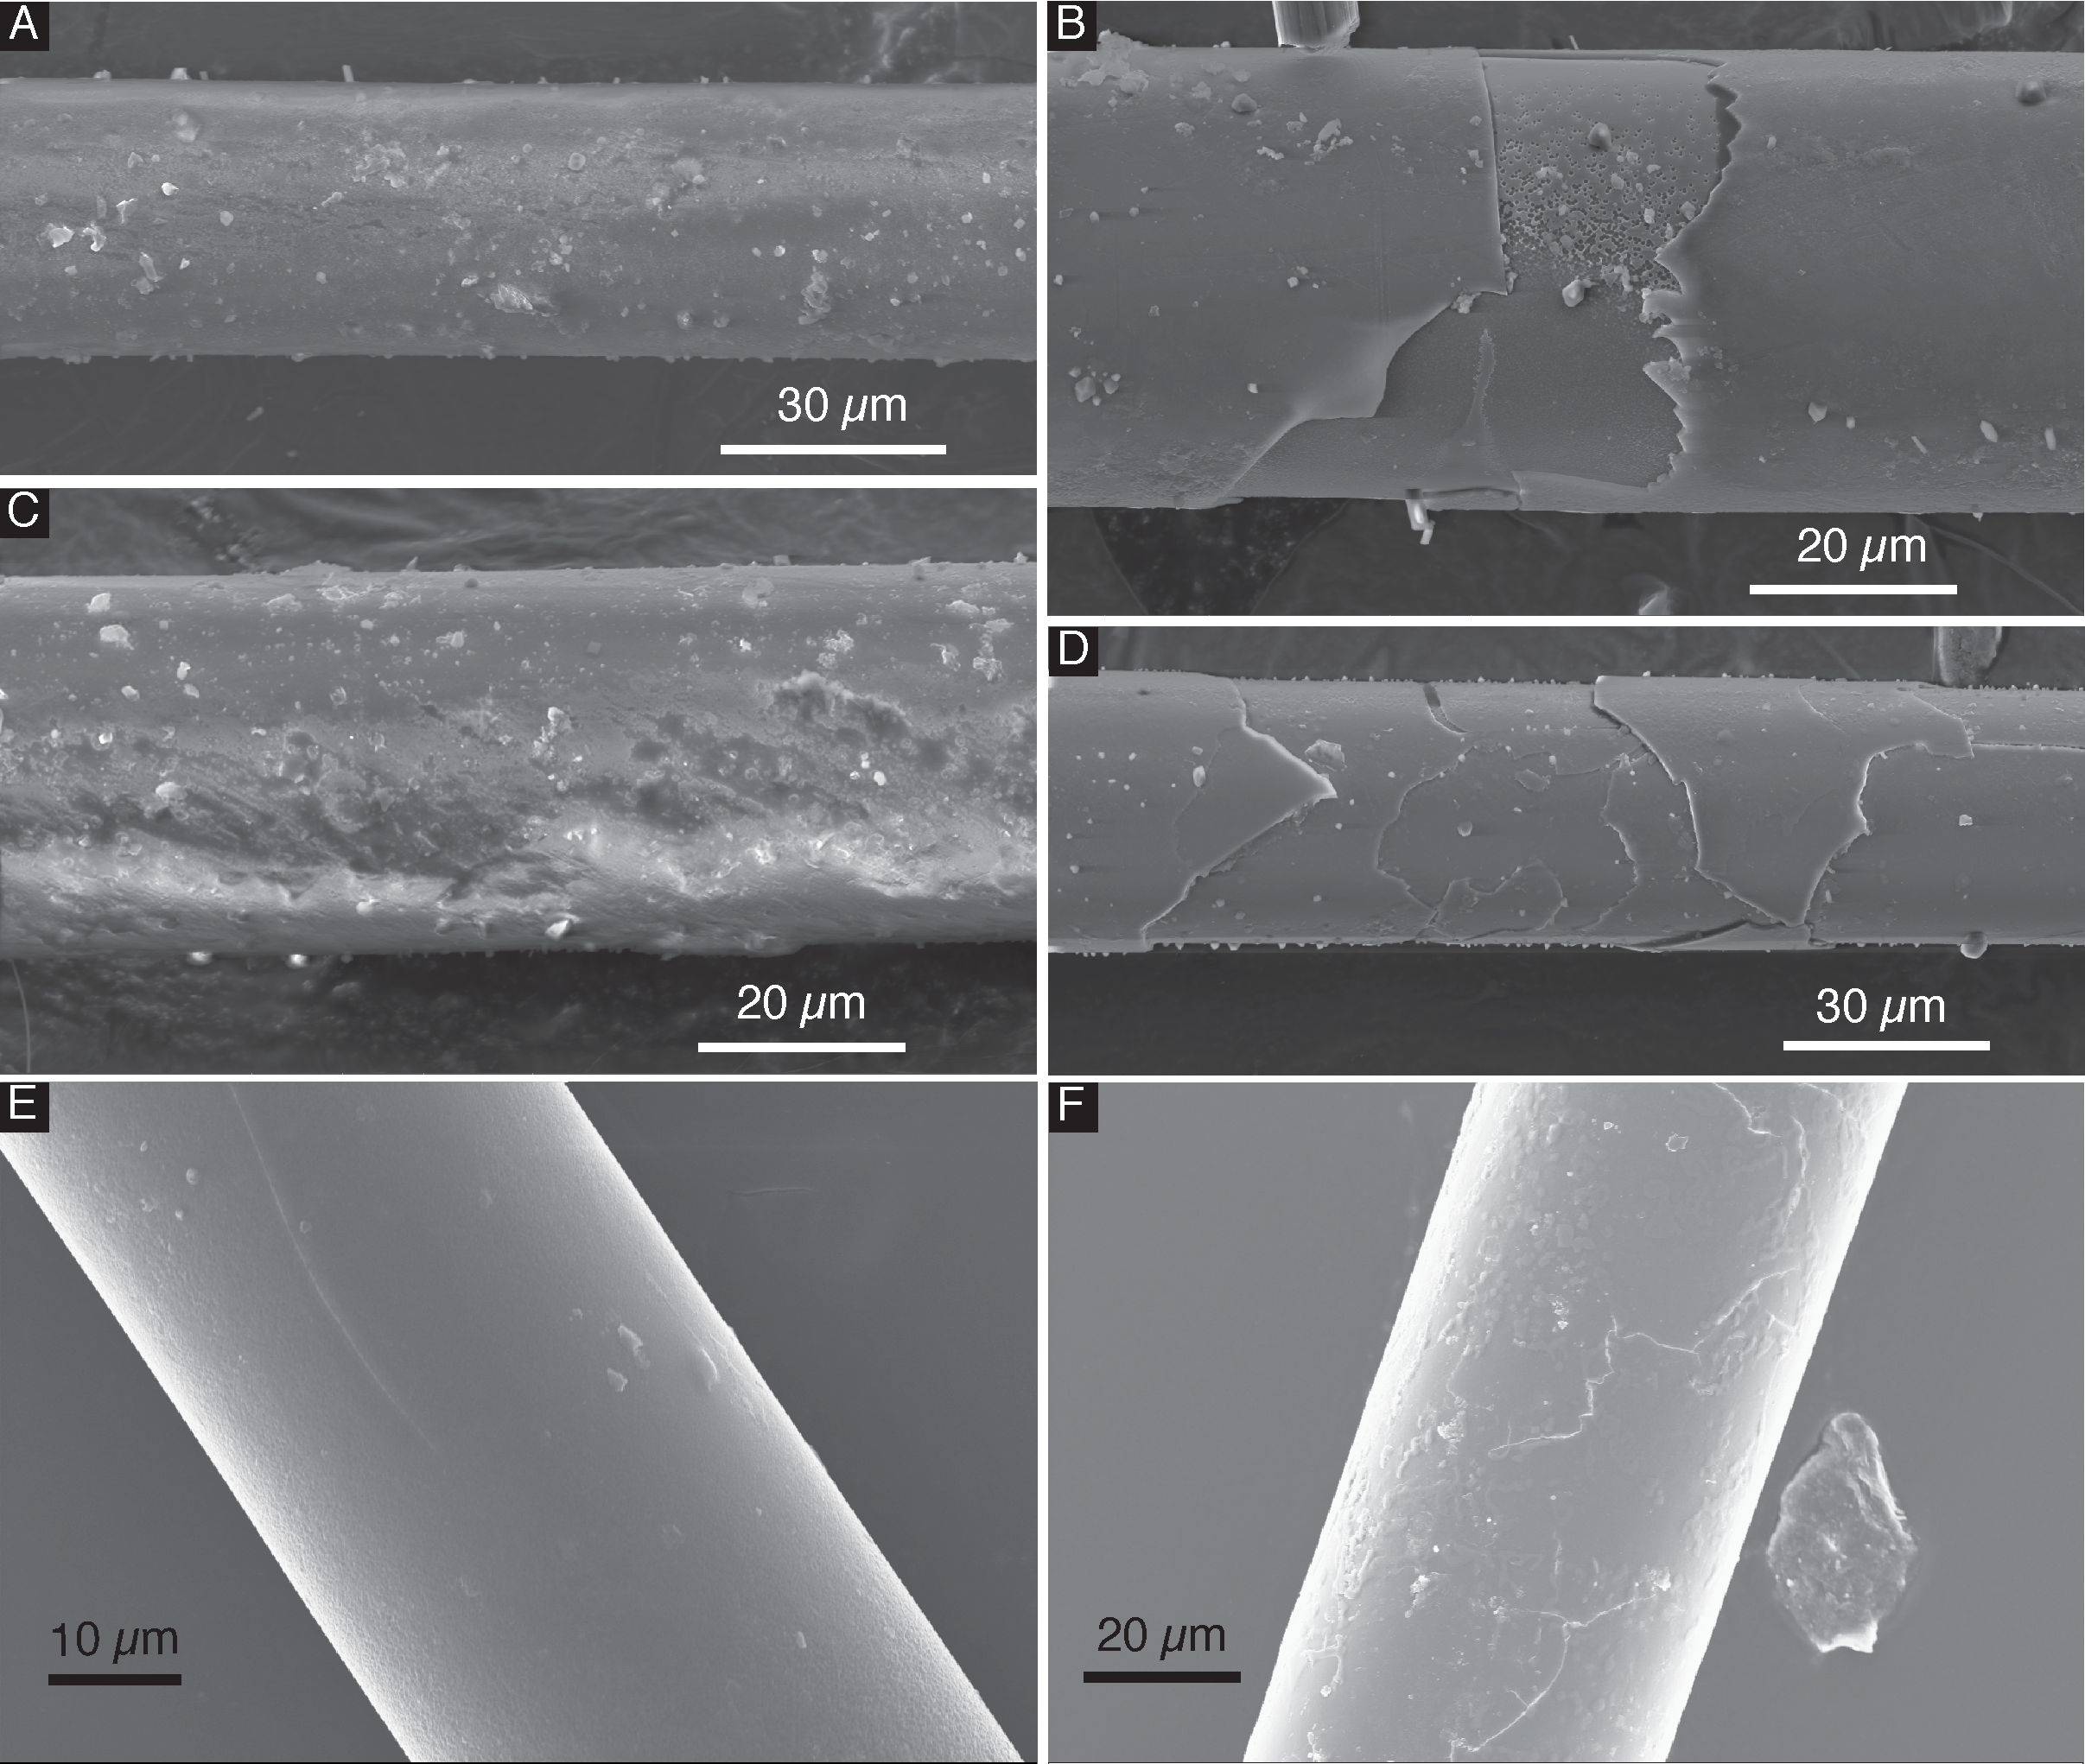
\includegraphics[width=0.9\textwidth]{Figures/EA_SEM.pdf}
\caption{SEM representative images of lateral surfaces of randomly selected \textit{Ea.} spicules after single load-unload simply-supported tests.
(\textsf{A}) and (\textsf{B}) show two different views of the same spicule whose Test No. is SS4 in Table~\ref{tab:SSdata_a}.
The Test No. for spicule in (\textsf{C}) is SS7.
The Test No. for spicule in (\textsf{D}) is SS24.
The Test No. for spicule in (\textsf{E}) is SS32.
The Test No. for spicule in (\textsf{F}) is SS34.
Both the spicules and the imaged region are chosen randomly.
All images are taken after the conclusion of single load-unload simply-supported tests.
}
\label{fig:SEM}
\end{figure}
